\documentclass[12pt]{report}
\usepackage{fullpage}
\usepackage{amssymb}
\usepackage{amsmath}
\usepackage{enumitem}
\usepackage{graphicx}
\usepackage{float}
\usepackage[colorlinks,citecolor=DeepPink4,linkcolor=DarkRed‌​]{hyperref}
\usepackage{url}
\usepackage{listings}
\usepackage{color}



\usepackage[utf8]{inputenc}
\usepackage{textcomp}
\usepackage{mathtools}
\usepackage{amsmath}
\usepackage{fancyhdr}

\pagestyle{fancy}
\fancyhf{} % clear all header and footer fields
\rfoot{https://github.com/afollestad/material-dialogs/issues/1162}
\renewcommand{\headrulewidth}{0pt}
\renewcommand{\footrulewidth}{0pt}
% each section on new page
\usepackage{etoolbox}
\pretocmd{\section}{%
  \ifnum\value{section}=0 \else\clearpage\fi
}{}{}

\definecolor{dkgreen}{rgb}{0,0.6,0}
\definecolor{gray}{rgb}{0.5,0.5,0.5}
\definecolor{mauve}{rgb}{0.58,0,0.82}
\lstset{frame=tb,
  language=Java,
  aboveskip=3mm,
  belowskip=3mm,
  showstringspaces=false,
  columns=flexible,
  basicstyle={\small\ttfamily},
  numbers=none,
  numberstyle=\tiny\color{gray},
  keywordstyle=\color{blue},
  commentstyle=\color{dkgreen},
  stringstyle=\color{mauve},
  breaklines=true,
  breakatwhitespace=true,
  tabsize=3
}





\renewcommand{\familydefault}{\sfdefault} % change font family to sans serif

\begin{document}

\title{Software Analytics - Bug details}
\author{Talal El Afchal}
\date{\today}
\maketitle
  \section*{Bug}
\href{https://github.com/afollestad/material-dialogs}{Material$-$dialogs} is an Android customizable dialogs API. The Git repository has 8758 $\star$ and 1440 commits.
The framework provides many types of dialog window, one of them is the \emph{Basic list} dialog which consists of a list of items and one check-box as shown in figure 1

\begin{figure}[H]
  \centering
  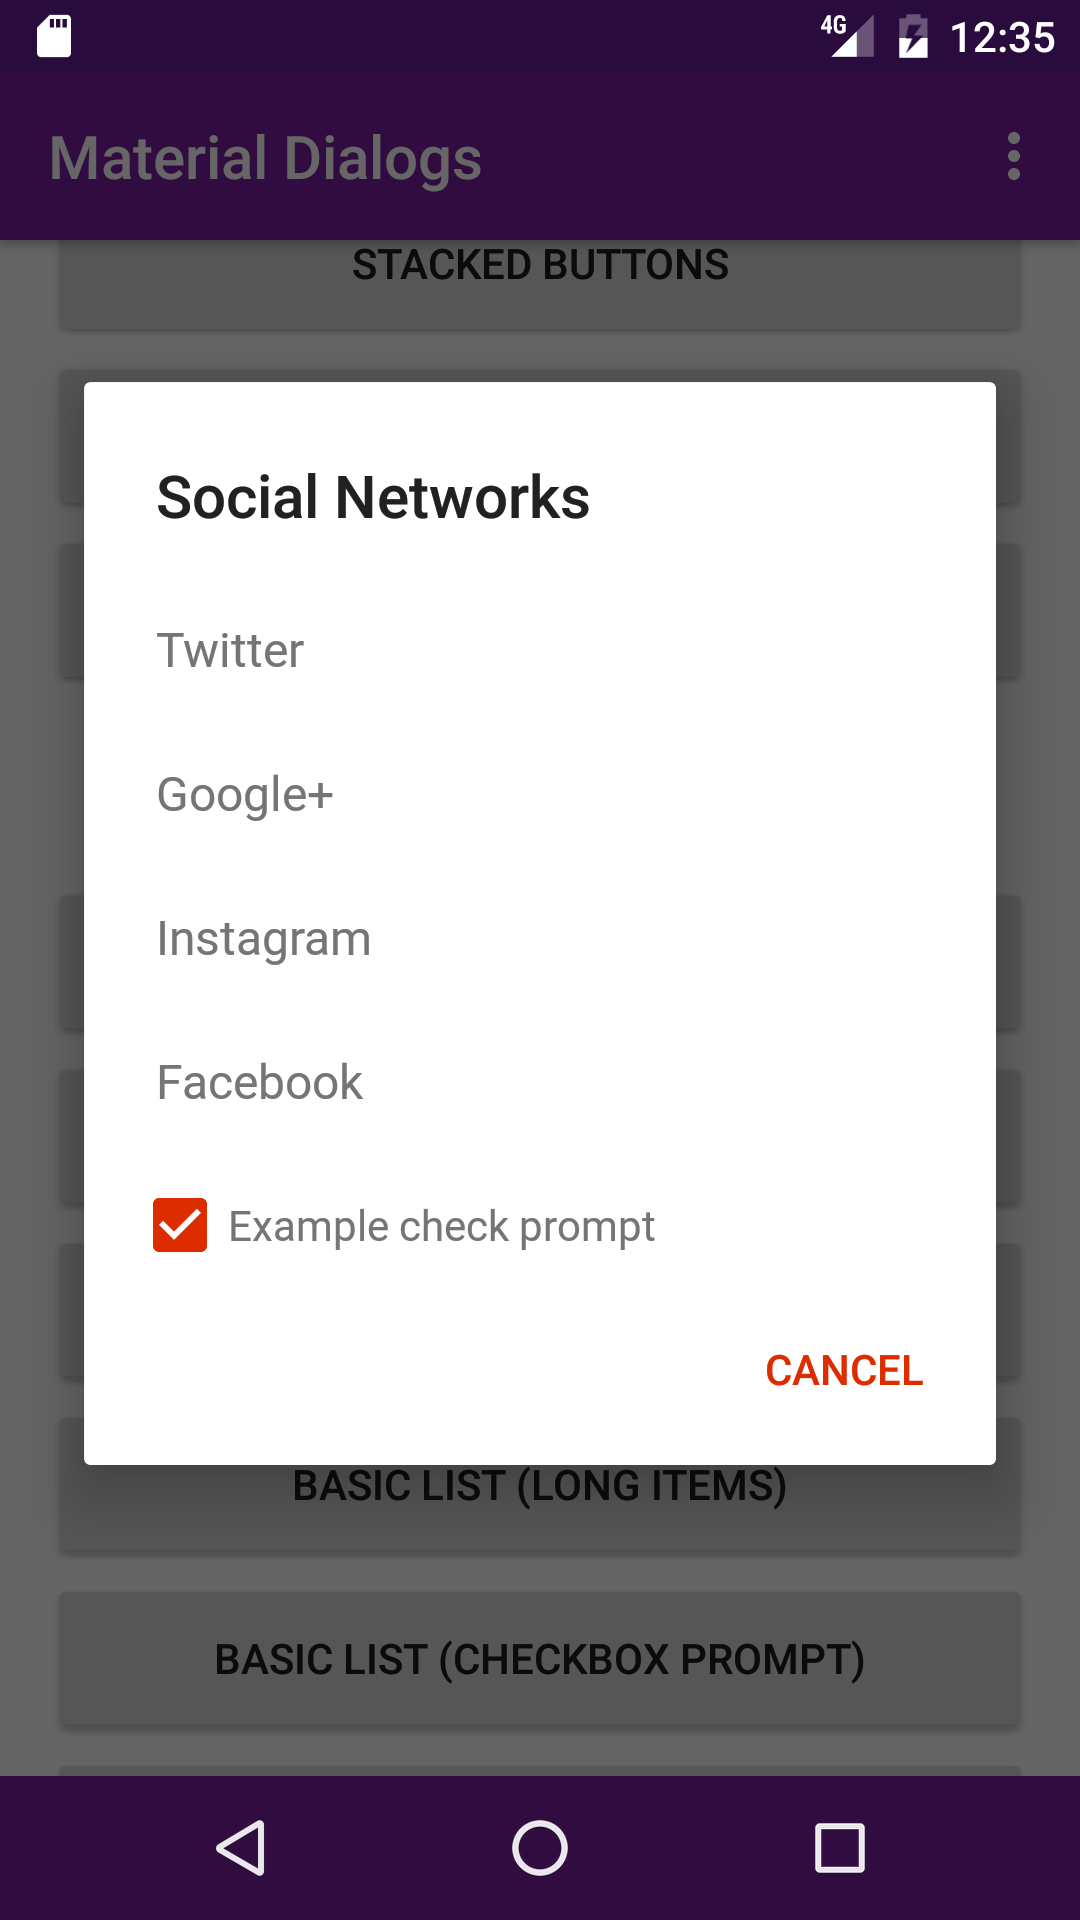
\includegraphics[height=0.4\textwidth]{screenshots/portrait.png}
  \caption{portrait}
\end{figure}
\noindent When the phone is in the landscape mode the check-box disappears as shown in figure 2, but the check-box must be visible like it is in the portrait mode.\\ On November 4, 2016 a \href{https://github.com/afollestad/material-dialogs/issues/1162}{\emph{``bug''}} label was added and on Jan 4, 2017 a \emph{``help wanted''} label was also added.\\


\begin{figure}[H]
  \centering
  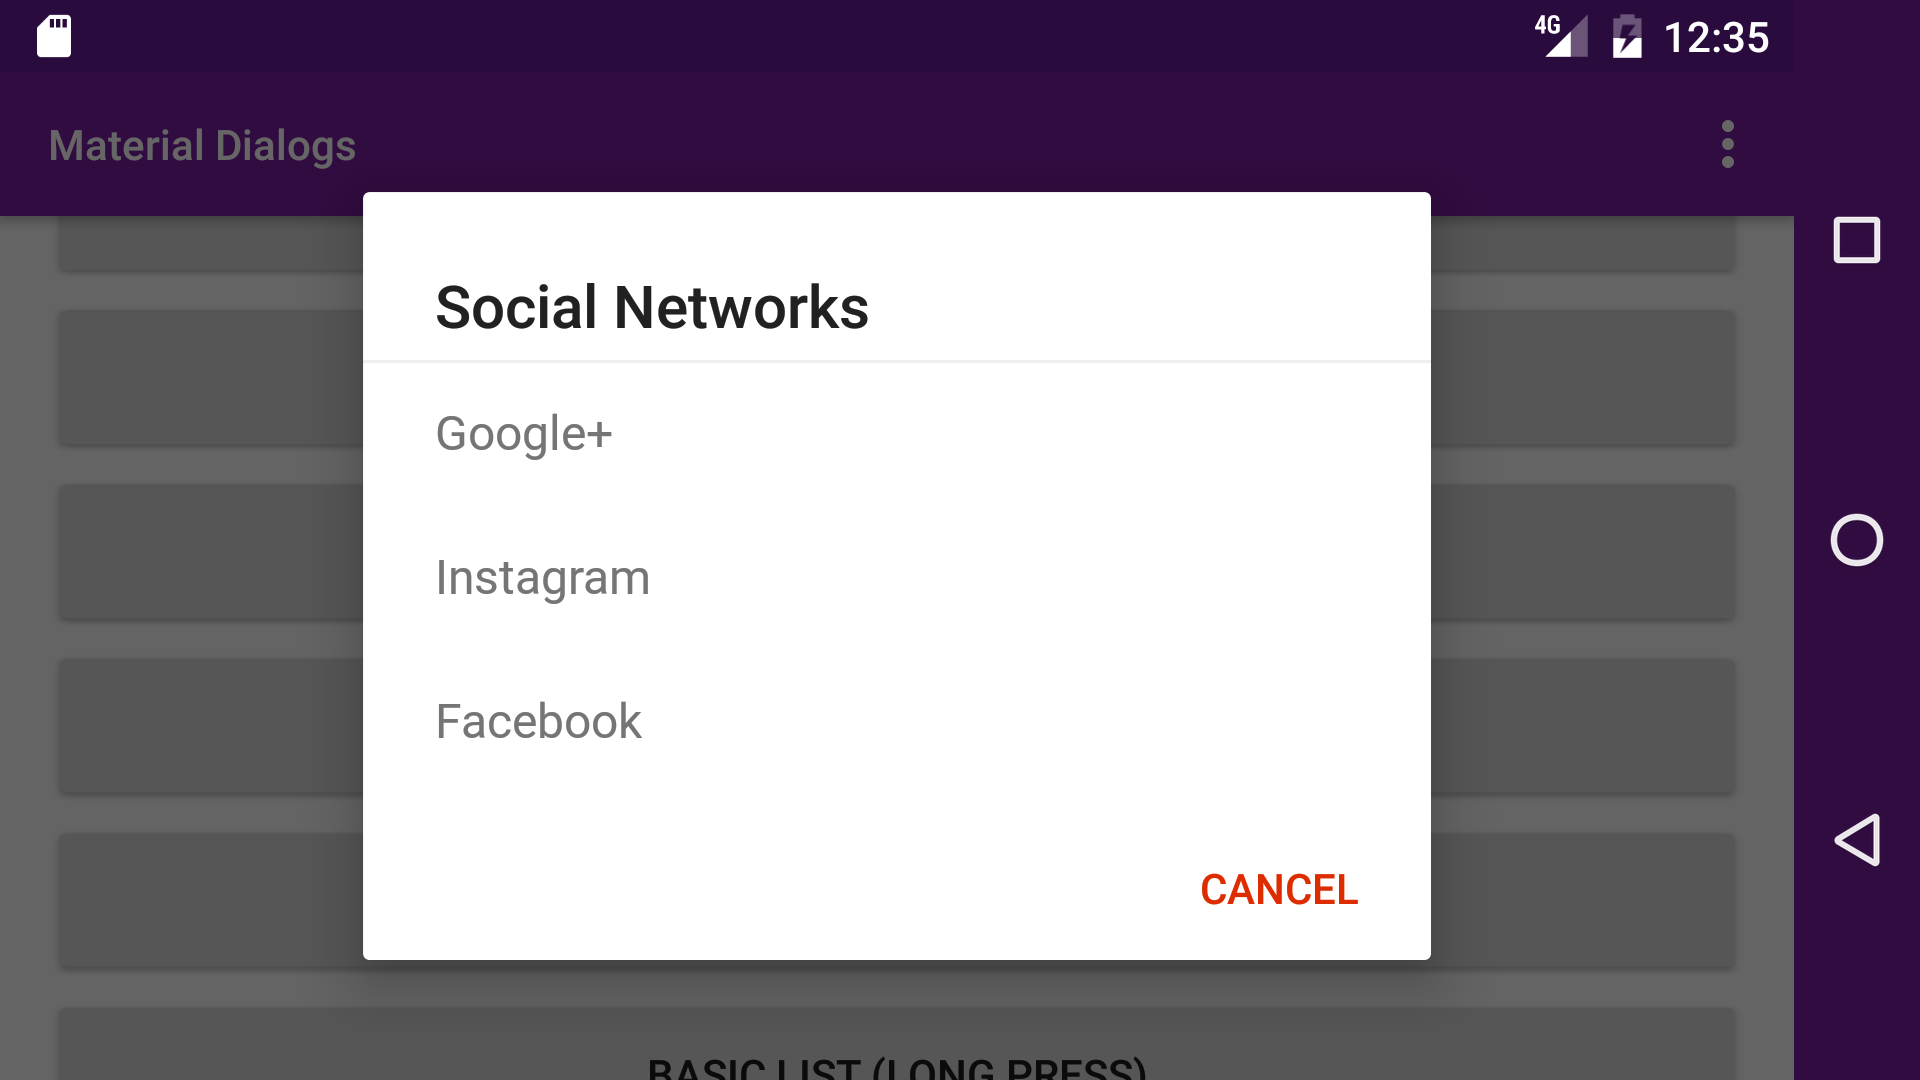
\includegraphics[width=0.6\textwidth]{screenshots/landscape.png}
  \caption{landscape}
\end{figure}


\section*{Bug replication}
  As mentioned in the last report, the check-box in the dialog list disappears when the phone is in landscape mode. Therefore the bug is visible and can by replicated as shown in the previous report.


\section*{Bug localization}
  In order to localize the bug, the first step is to open the project in Android Studio and then from the main activity xml file we can retrieve the id of the \emph{BASIC LIST(CHECKBOX PROMPT)} button, that generates the dialog list in which we are interested, as shown in figure 1.
\begin{figure}[H]
  \centering
  \includegraphics[width=0.6\textwidth]{screenshots/id.png}
  \caption{Android Studio}
\end{figure}
\noindent
  The next step is to use the id to figure out which method is implementing the button's functionality.\\ 
  I found that the method \emph{showListCheckPrompt()} in \emph{Main Activity} class is called when the button is clicked. This method creates an object of type \emph{MaterialDialog.Builder} (Builder is an inner class), and several methods are invoked on this object as shown in the snippet code. My first guess is that the bug is located in the \emph{show()} method since it shows the check-box in the dialog window.

  \begin{lstlisting}
    @OnClick(R.id.list_checkPrompt) public void showListCheckPrompt() {
        new MaterialDialog.Builder(this)
                .title(R.string.socialNetworks)
                .items(R.array.socialNetworks)
                .itemsCallback((dialog, view, which, text) -> showToast(which + ": " + text))
                .checkBoxPromptRes(R.string.example_prompt, true, null)
                .negativeText(android.R.string.cancel)
                .show();
    }
\end{lstlisting}
\noindent
  Performing a deeper analysis, \emph{show()} is invoked 31 times on 31 different \emph{MaterialDialog} objects and it is invoking the \emph{show()} method from \emph{MaterialDialog} class which is invoking the android API \emph{show()} method. Since the bug is not replicated in these 31 objects and must probably the bug is not in the Android API, I moved my focus to the other methods.\\
  The next step is to analyze the \emph{checkBoxPromptRes()} method. This method sets the attributes of the checkBox variable of a MaterialDialog object. Performing a deeper analysis the \emph{DialogInit} class maps this variable to the xml file. This path leads us to \emph{md\_dialog\_list\_check.xml} file where I spot the bug.\\
  By removing the items list, the check-box is visible in the landscape mode, as we can see in Figure 2 . My conclusion is that the \emph{ScrollView} is hiding the check-box and this why we can't see both of them in the landscape mode.
  \begin{figure}[H]
  \centering
  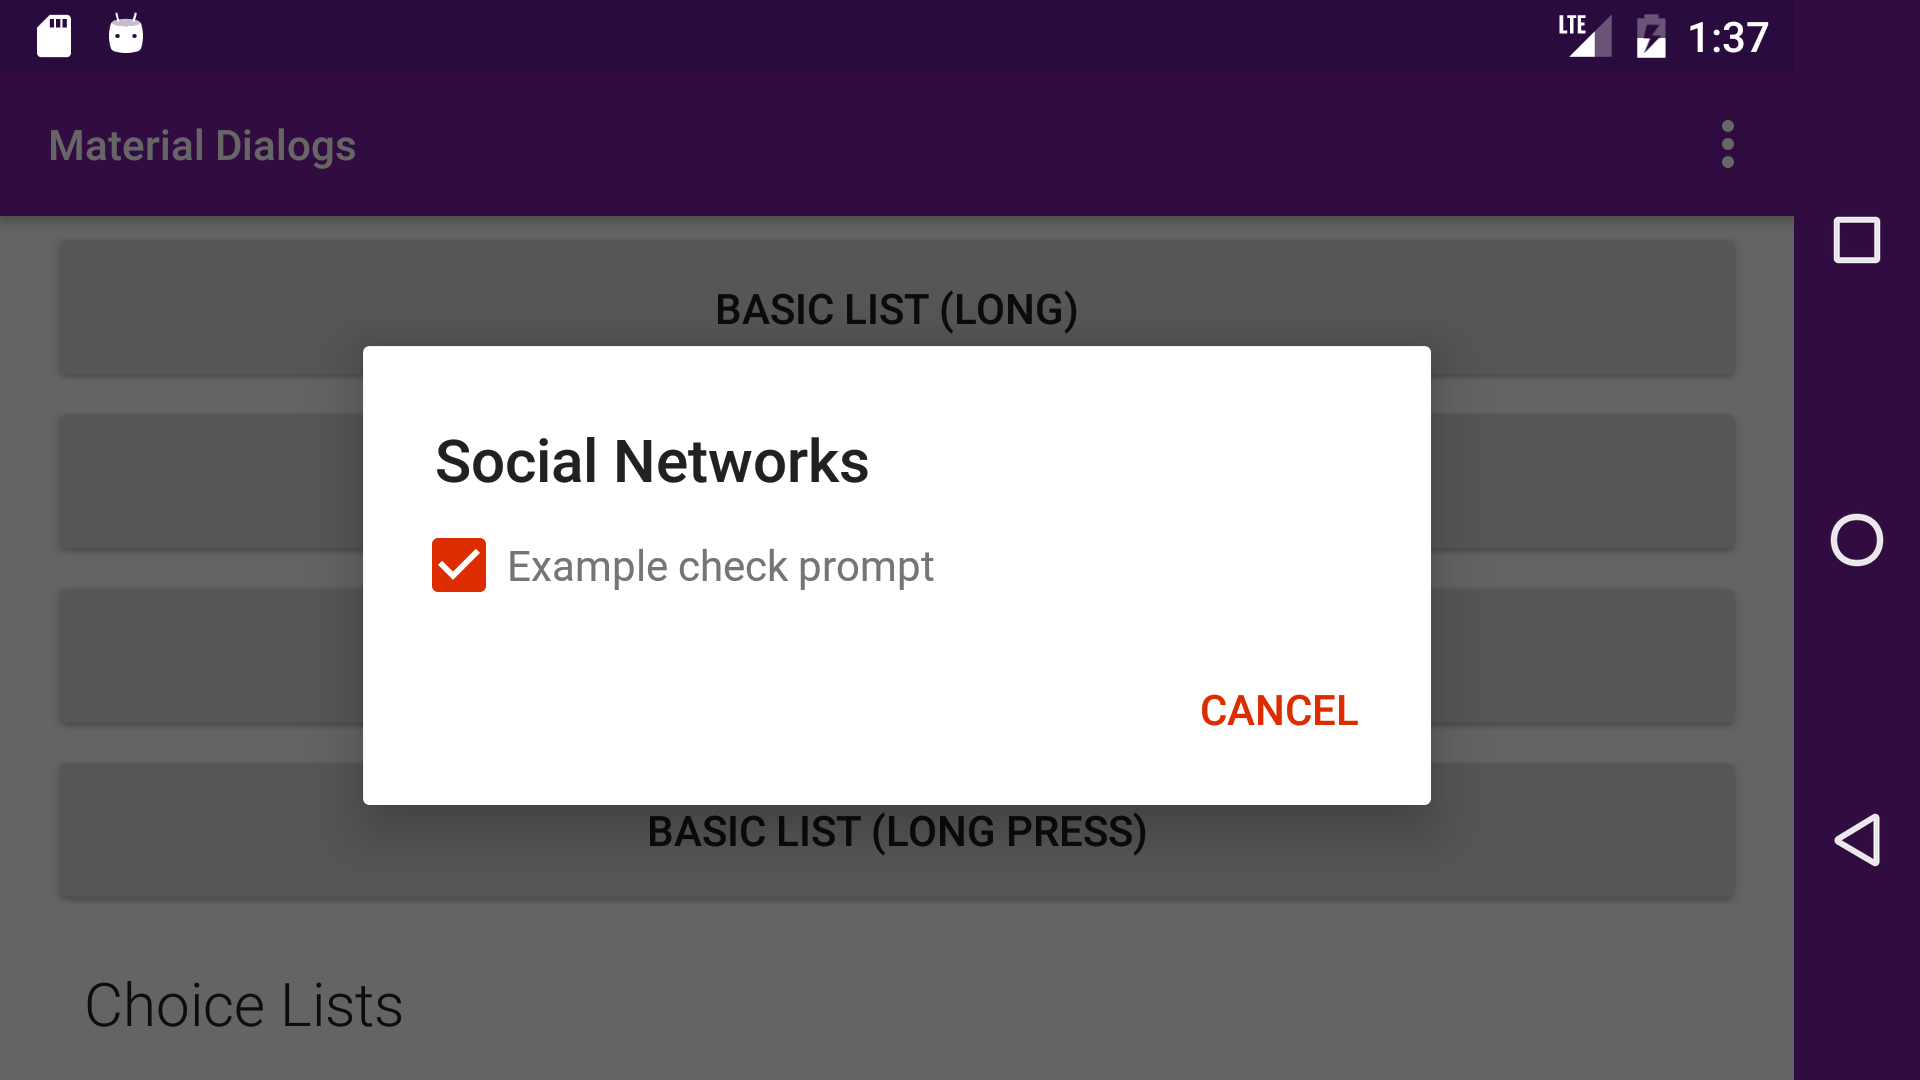
\includegraphics[width=0.6\textwidth]{screenshots/checkbox.png}
  \caption{Check box}
\end{figure}

\section*{Changes impact}
The \emph{md\_dialog\_list\_check.xml} file creates the \emph{BASIC LIST (CHECK BOX PROMPT)}`s window interface only. If we make changes in this file, the changes will not affect other dialog windows or other files.
 

\section*{Plan}
My plan is to create 2 layouts, one for the scroll-view and one for the check-box, instead of having them in the same layout.

\end{document}








